\subsection{Comportamiento electroquímico}

\subsubsection{Cambio de volumen fraccionario}

\begin{figure}[t]
    \centering
    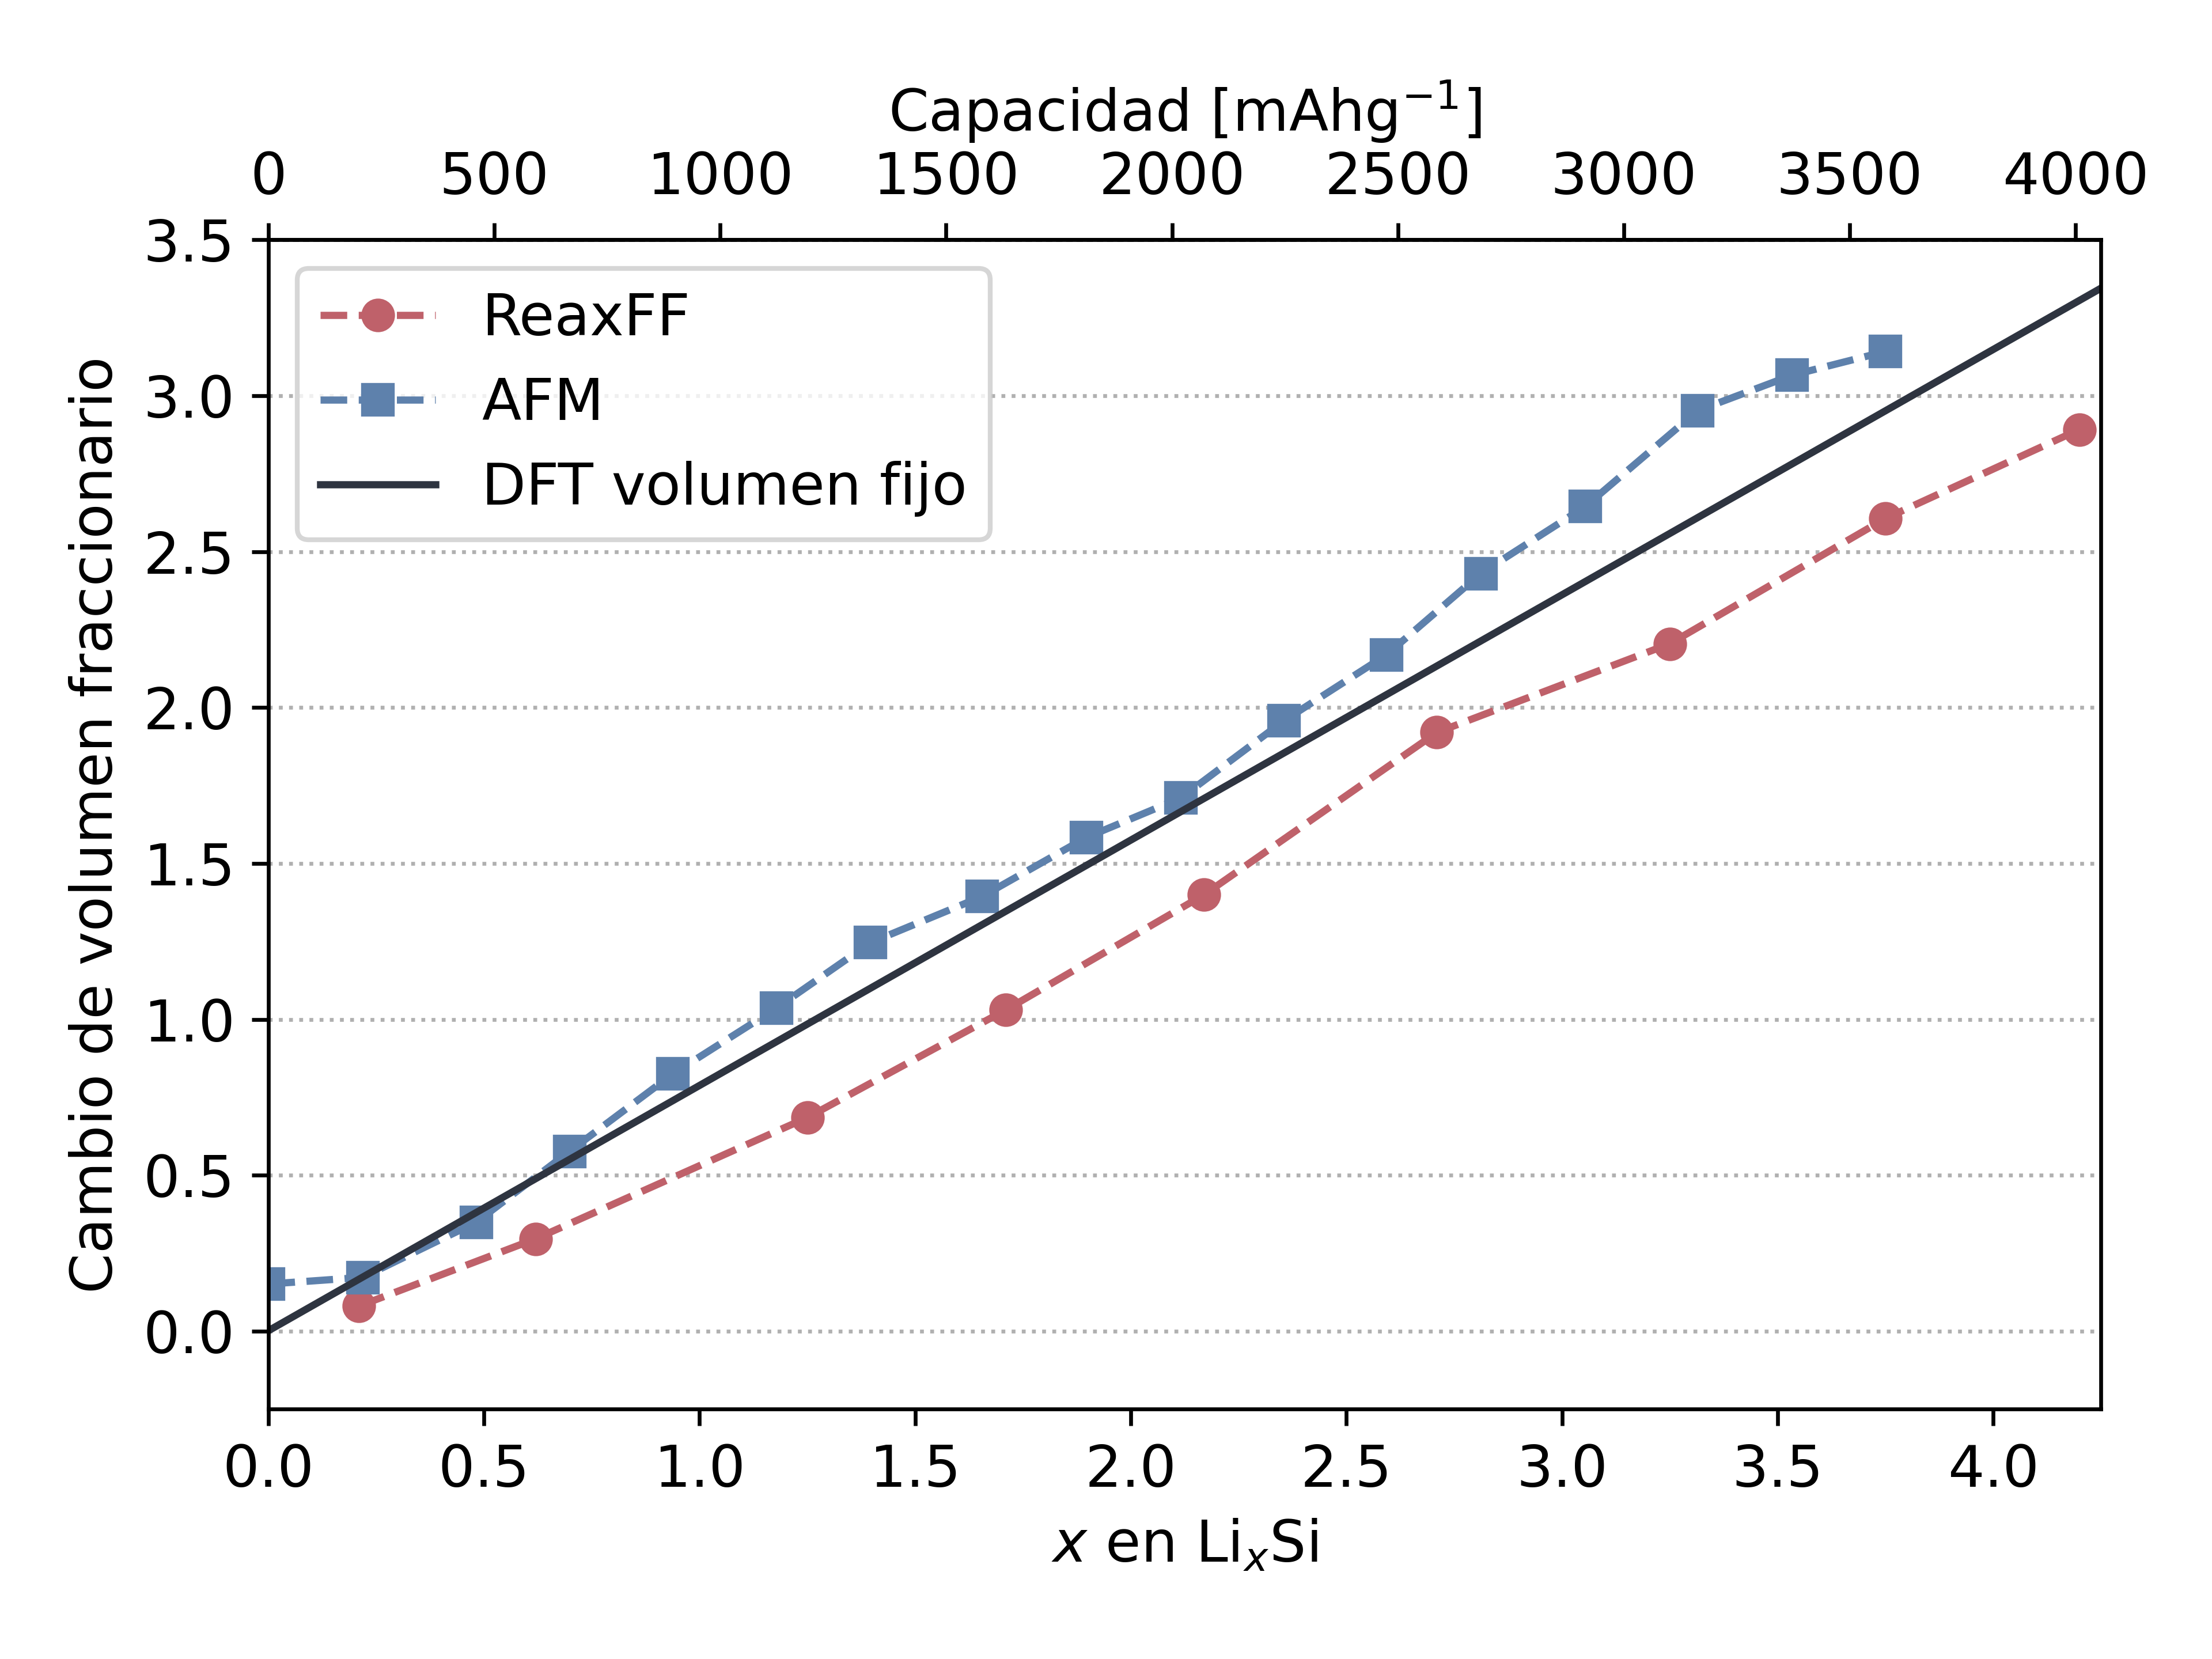
\includegraphics[width=0.8\textwidth]{Silicio/caracterizacion/resultados/electroquimica/fvc.png}
    \caption{Cambio de volumen fraccionario en función de la composición de la 
    aleación. Los valores experimentales de AFM se muestran con cuadrados azules, 
    la línea recta se corresponde con cálculos de DFT y los círculos naranjas son 
    resultados de este trabajo.}
    \label{fig:fvc}
\end{figure}
El cambio de volumen fraccionario puede definirse utilizando una normalización 
relativa al número de átomos de Si en la estructura de acuerdo a
\begin{equation}\label{eq:fvc}
    \text{fvc} = \frac{N_{\text{Si}}}{V_{\text{Si}}} \left( \frac{V_{\text{Si},x}}{N_{\text{Si},x}} - \frac{V_{\text{Si}}}{N_{\text{Si}}} \right),
\end{equation}
donde $V_{\text{Si}}$ y $N_{\text{Si}}$ son el volumen y el número de átomos de 
Si en la celda unidad de c-Si, $V_{\text{Si},x}$ y $N_{\text{Si},x}$ son el 
volumen y el número de átomos de Si
en la celda de simulación para el valor correspondiente de $x$. En la Figura
\ref{fig:fvc} se muestran los valores calculados a partir de la ecuación 
\ref{eq:fvc} para las distintas estructuras de Li$_x$Si estudiadas. En la misma 
se comparan los valores obtenidos con datos experimentales de AFM (\textit{atomic 
force microscopy}, sus siglas en inglés) medidos por Beaulieu \textit{et al.} 
~\cite{beaulieu2003} y con valores de DFT fijos de cambio volumétrico utilizado 
por Chevrier y Dahn ~\cite{chevrier2009}. Los mismos muestran que el
potencial ReaxFF proporciona una tendencia correcta, tanto cualitativa como 
cuantitativamente.

\subsubsection{Voltaje}

\begin{table}[b]
    \centering
    \caption{Energías de formación obtenidas a través de la ecuación \ref{eq:fe}}
    \setlength\extrarowheight{2pt}\stackon{%
    \begin{tabular}{c c}
        \toprule
        \textbf{x en Li$_x$Si} & 
        \textbf{Energía de formación [eV]} \\ 
        \midrule
        0.21  &  0.503 $\pm$ 0.003 \\
        0.62  &  0.121 $\pm$ 0.007 \\
        1.25  & -0.12 $\pm$ 0.01 \\
        1.71  & -0.236 $\pm$ 0.007 \\
        2.17  & -0.355 $\pm$ 0.008 \\
        2.71  & -0.410 $\pm$ 0.007 \\
        3.25  & -0.52 $\pm$ 0.01 \\
        3.75  & -0.62 $\pm$ 0.01 \\
        4.20  & -0.699 $\pm$ 0.008 \\
        \bottomrule
    \end{tabular}
    }{}
    \label{t:fe}
\end{table}
Las energías obtenidas pueden ser utilizadas para evaluar el funcionamiento del 
modelo para predecir propiedades electroquímicas, como fue sugerido por Chevrier
y Dahn ~\cite{chevrier2009}. Primero, se define la energía de formación de las 
distintas estructuras amorfas como
\begin{equation}\label{eq:fe}
    E_f(x) = E_{\text{Li}_x\text{Si}} - (x E_{\text{Li}} + E_{\text{Si}}),
\end{equation}
donde $E_{\text{Li}_x\text{Si}}$ es la energía de la aleación Li$_x$Si por átomo 
de Si, $E_{\text{Li}}$ y $E_{\text{Si}}$ son las energías cohesivas de Li y Si
en sus fases cristalinas. Usando
la ecuación \ref{eq:fe} como aproximación a la energía de formación de Gibbs, el 
potencial \textit{versus} Li metálico de Li$_x$Si puede obtenerse a partir de
\begin{equation}\label{eq:voltaje}
    V(x) = - \frac{dE_f(x)}{dx},
\end{equation}
donde $V$ es el potencial. Los datos obtenidos así pueden compararse con valores
experimentales y computacionales previos. Las energías de formación calculadas
a partir de la ecuación \ref{eq:fe} se muestran en la Tabla \ref{t:fe}. 
Si se realiza un \textit{spline} a estos valores, mostrados en el recuadro de la
Figura \ref{fig:voltaje}, se obtienen los valores de $V(x)$ a partir de la ecuación
\ref{eq:voltaje}, que se grafican en función de la composición en la Figura 
\ref{fig:voltaje} con una línea naranja. Para comparar, se incluyen en la misma Figura
las curvas experimentales medidas para la litiación y la delitiación de silicio
amorfo ~\cite{hatchard2004} y la curva teórica de cálculos de primeros principios 
~\cite{chevrier2009}. Se puede afirmar que los resultados obtenidos con el ReaxFF 
son satisfactorios.

\begin{figure}[h]
    \centering
    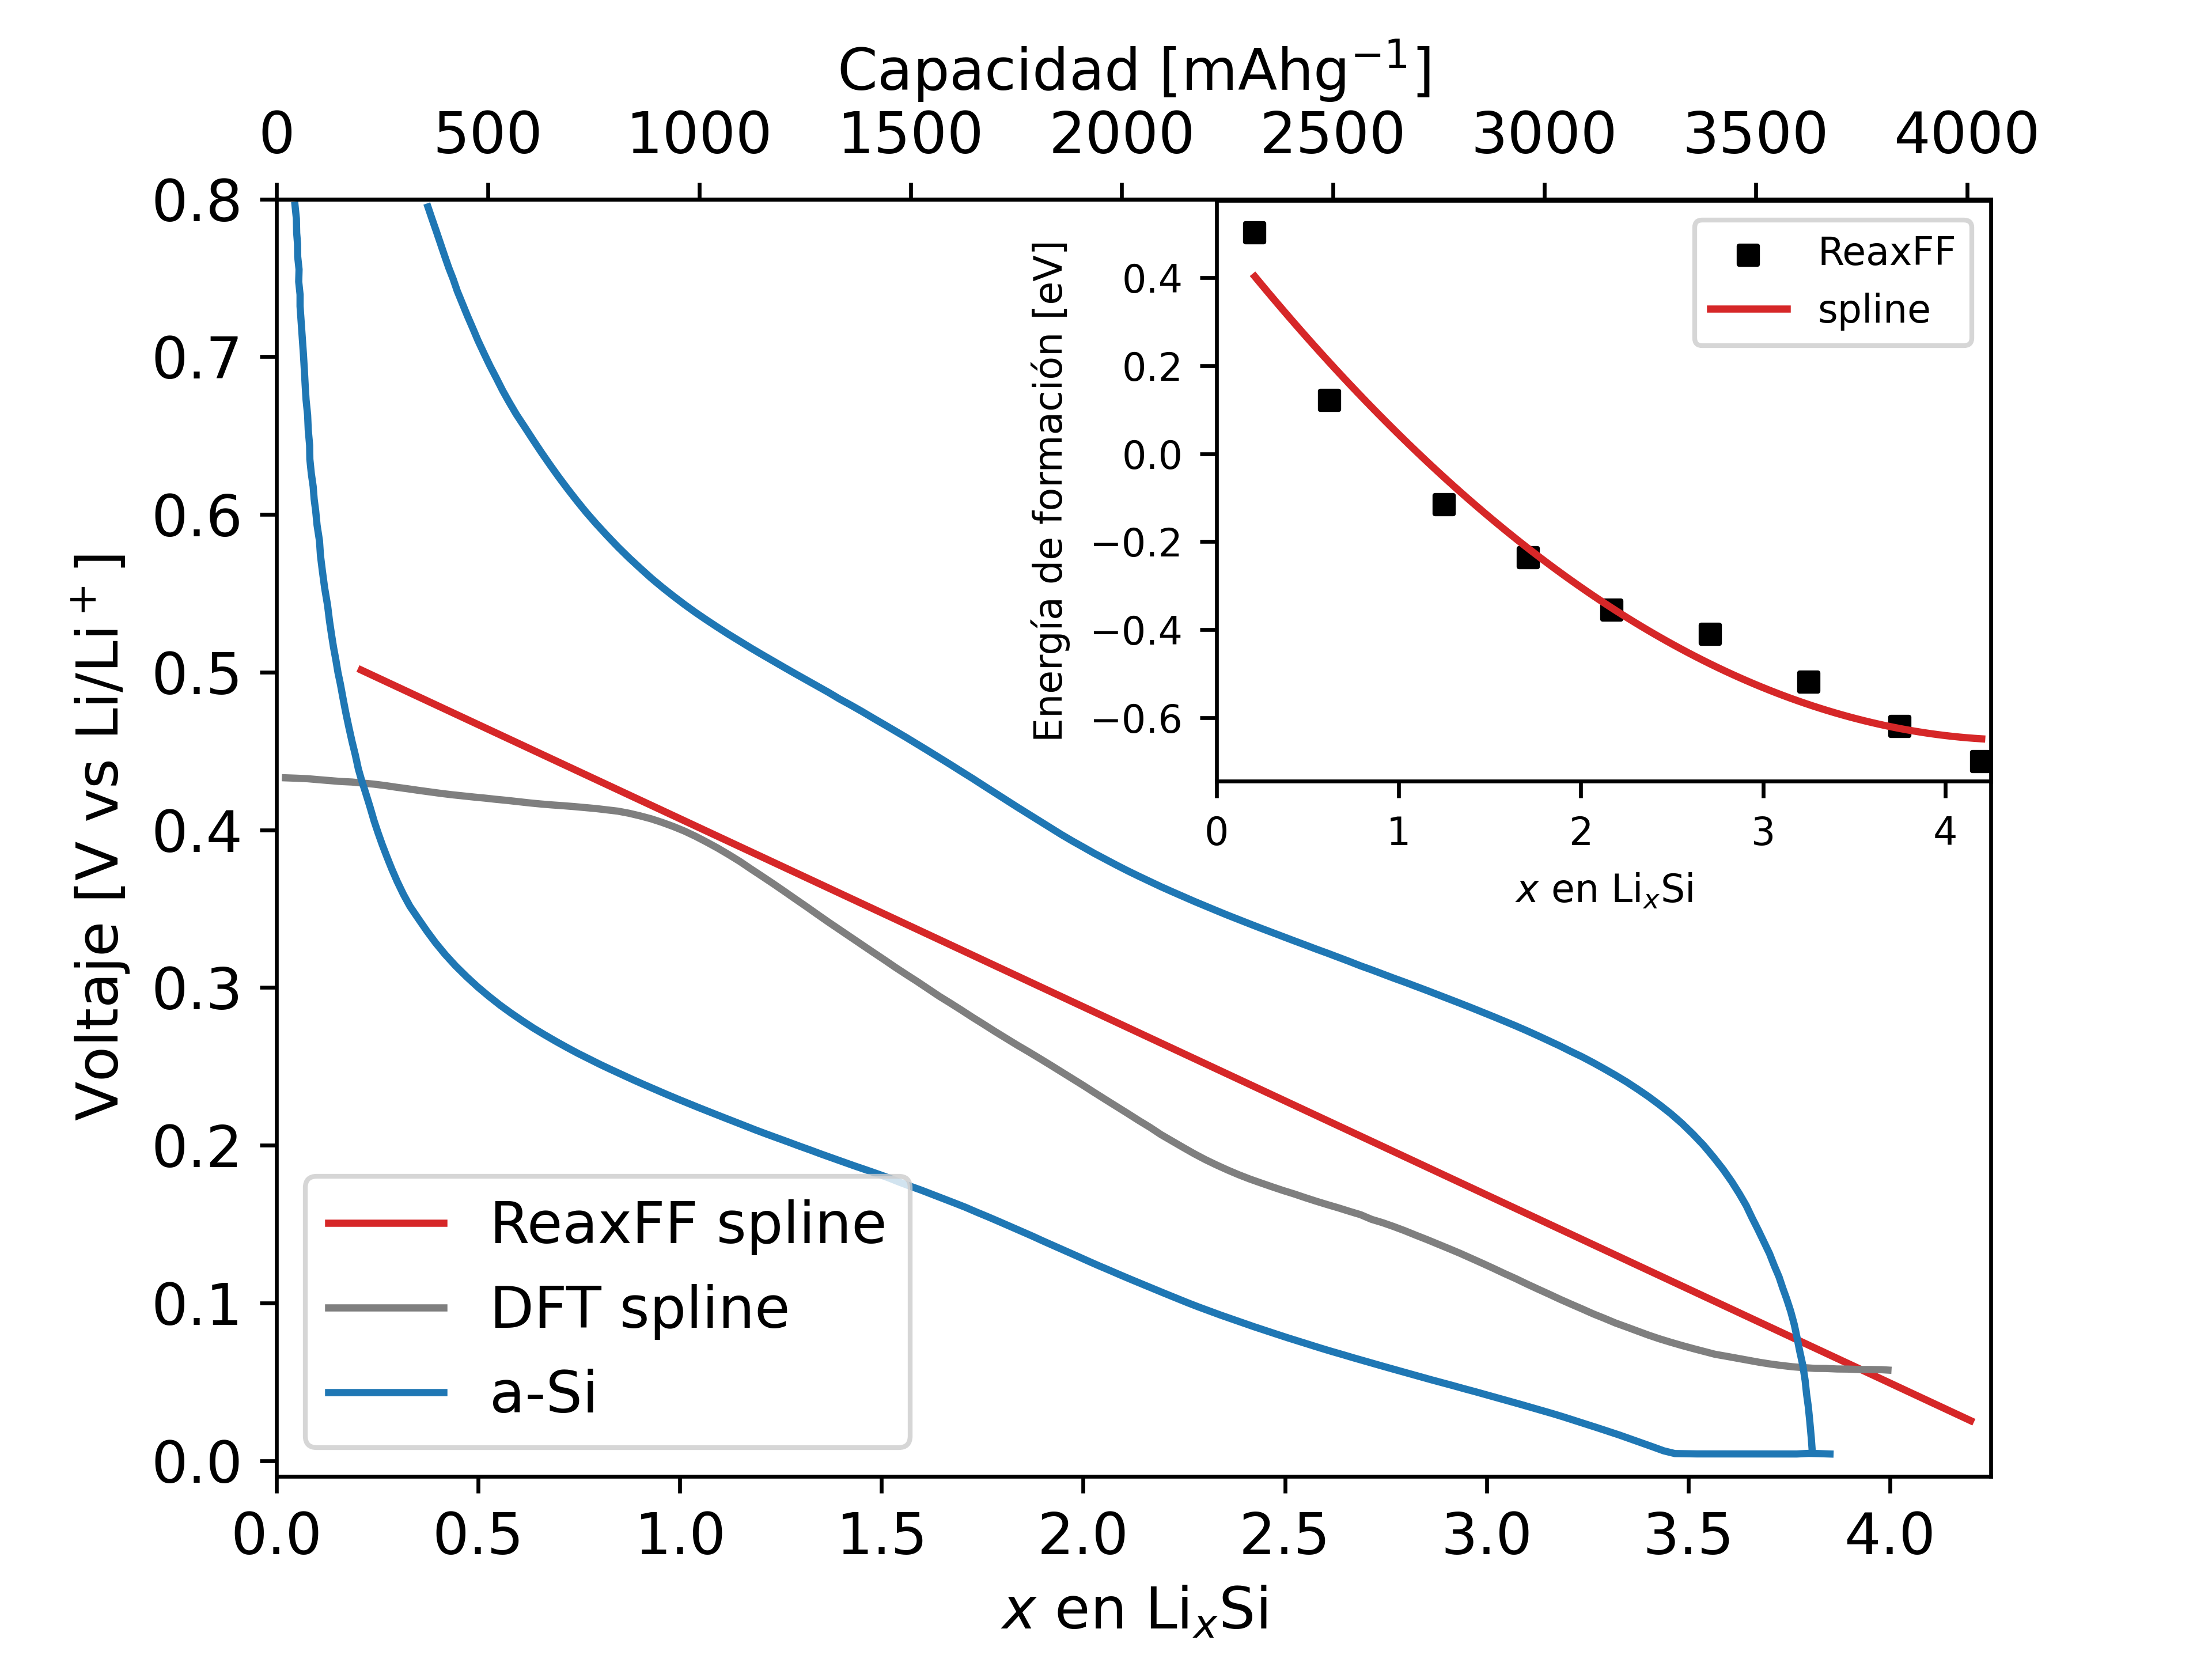
\includegraphics[width=0.8\textwidth]{Silicio/caracterizacion/resultados/electroquimica/voltaje.png}
    \caption{Curvas potencial-concentración para la litiación de ánodos de Si.
    La línea negra corresponde a cálculos de DFT, las líneas azules a 
    curvas medidas experimentalmente en la litiación de Si amorfo y la línea 
    roja es la derivada del \textit{spline} ajustado a los datos de la energía 
    de formación obtenidos con el ReaxFF, presentados en el recuadro.}
    \label{fig:voltaje}
\end{figure}
